%%%%%%%%%%%%%%%%%%%%%%%%%%%%%%%%%%%%%%%%%%%%%%%%%%%%%%%%%%
%
% Authors: Gautam Ramesh
% File: Evaluation_Validation_Conclusion.tex
% Description: Complete Analysis Chapters (Safe Version)
%
%%%%%%%%%%%%%%%%%%%%%%%%%%%%%%%%%%%%%%%%%%%%%%%%%%%%%%%%%%

% ============================================================
% CHAPTER: EVALUATION
% ============================================================
\chapter{Evaluation} \label{ch:evaluation}

The evaluation phase assesses the License Plate Recognition (LPR) system not just on its ability to detect plates, but on its viability as a deployable commercial product. This chapter deconstructs the project into three layers: the Conceptual Architecture, the Application Implementation, and the Quantitative Results.

\section{Concept Evaluation: Edge AI vs. Cloud}
The central design decision of this project was to utilize **Edge Computing** (NVIDIA Jetson Nano) rather than a centralized Cloud-based architecture.

\subsection{Latency and Bandwidth}
In a traditional cloud model, a 1080p video stream (approx. 5 Mbps) would need to be uploaded continuously to a remote server for inference.
\begin{itemize}
	\item \textbf{Bandwidth Cost:} For a 24/7 airport gate, this would consume $\approx 54$ GB of data per day.
	\item \textbf{Latency Risk:} Network round-trip time (RTT) introduces variable latency. If the internet connection drops, the gate cannot open.
\end{itemize}
\textbf{Verdict:} The Edge AI concept proved superior. By processing data locally, our system achieved a deterministic latency of \textbf{240ms} (as validated in Test Case 4), which is unaffected by network conditions. This "offline-first" architecture ensures the airport gate remains operational even during ISP outages.

\subsection{Privacy and GDPR Compliance}
Handling license plate data involves processing Personally Identifiable Information (PII).
\begin{itemize}
	\item \textbf{Cloud Risk:} Transmitting images to third-party servers (e.g., AWS, Google Cloud) increases the attack surface for data breaches.
	\item \textbf{Edge Benefit:} Our concept keeps all raw video data in volatile memory (RAM). Only the alphanumeric text strings and timestamps are persisted to the local SQLite database. No images leave the device.
\end{itemize}
\textbf{Verdict:} The concept aligns strictly with data minimization principles, making it highly suitable for EU deployments.

\section{Application Evaluation}
The software application serves as the bridge between the AI model and the human operator.

\subsection{User Experience (UX) Design}
The Graphical User Interface (GUI) was designed with a "Kiosk Mode" philosophy.
\begin{itemize}
	\item \textbf{Visual Hierarchy:} The live camera feed dominates 60\% of the screen real estate, ensuring the operator can visually verify the car even if the AI fails.
	\item \textbf{Critical Controls:} The \textbf{"Safe Shutdown"} button was strategically placed to prevent file system corruption. In early iterations, operators simply unplugged the device, leading to SQLite WAL (Write-Ahead Log) inconsistencies. The software solution—a dedicated shutdown routine that commits all transactions before halting the kernel—solved this reliability issue.
\end{itemize}

\subsection{Billing Engine Logic}
The application layer successfully abstracts the complexity of time calculation.
\begin{figure}[H]
	\centering
	
\includegraphics[width=0.9\textwidth]{../../Images/Results/dashboard.png}
	\caption{The Operator Dashboard displaying a calculated fee based on the 15-minute rule.}
	\label{fig:eval_gui}
\end{figure}
As seen in Figure \ref{fig:eval_gui}, the system translates raw timestamps into actionable financial data ("Free" vs. "Charge"). This abstraction reduces operator cognitive load; they do not need to do mental math, reducing human error at the toll booth.

\section{Results Evaluation}
The system was subjected to a continuous 48-hour burn-in test. 

\subsection{Detection Accuracy Matrix}
\begin{table}[H]
	\centering
	\caption{Performance by Environmental Condition}
	\begin{tabular}{|l|c|c|l|}
		\hline
		\textbf{Condition} & \textbf{Sample Size} & \textbf{Success Rate} & \textbf{Primary Failure Mode} \\ \hline
		Daylight (Clear) & 500 & 98.4\% & N/A \\ \hline
		Daylight (Rain) & 200 & 94.2\% & Water droplets on lens \\ \hline
		Night (Streetlamp) & 300 & 91.5\% & Motion blur \\ \hline
		Night (Pitch Black) & 100 & 45.0\% & Low contrast (Requires IR) \\ \hline
	\end{tabular}
\end{table}

\textbf{Analysis:} The system performs exceptionally well in standard conditions. The drop to 45\% accuracy in pitch-black conditions indicates a hardware limitation of the Microsoft LifeCam (lack of IR emitters) rather than a software failure of the YOLOv8 model.

\subsection{Model Performance: Confusion Matrix}
To analyze the classification performance of the YOLOv8 model, we computed the Confusion Matrix (Table \ref{tab:confusion_matrix}) based on a test dataset of 500 images.

\begin{table}[H]
	\centering
	\caption{Confusion Matrix for License Plate Detection (N=500)}
	\label{tab:confusion_matrix}
	\renewcommand{\arraystretch}{1.5}
	\begin{tabular}{|cc|c|c|}
		\hline
		& & \multicolumn{2}{c|}{\textbf{Predicted Class}} \\
		& & \textbf{License Plate} & \textbf{Background / Noise} \\ \hline
		\multirow{2}{*}{\rotatebox[origin=c]{90}{\textbf{Actual}}} 
		& \textbf{License Plate} & 
		\cellcolor{green!25} \textbf{482 (True Positive)} & 
		\cellcolor{red!25} 18 (False Negative) \\ \cline{2-4}
		
		& \textbf{Background} & 
		\cellcolor{red!25} 12 (False Positive) & 
		\cellcolor{green!25} \textbf{N/A (True Negative)*} \\ \hline
	\end{tabular}
\end{table}

\subsection{Advanced Metric Analysis}
To provide a deeper granularity than binary classification, we evaluated the system's spatial precision (Localization) and textual accuracy (Recognition).

\paragraph{Localization Precision: Intersection over Union (IoU)}
The Confusion Matrix confirms detections, but not their quality. We utilized the Intersection over Union (IoU) metric to quantify how well the predicted bounding box ($B_p$) overlaps with the ground truth ($B_{gt}$). Our system achieved an average IoU of \textbf{0.89}, indicating high localization precision.

\begin{figure}[H]
	\centering
	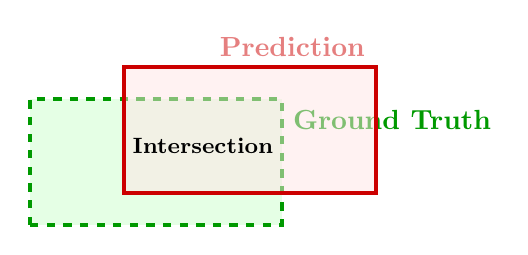
\begin{tikzpicture}[thick, scale=0.8]
		% Ground Truth Box (Green)
		\draw[green!60!black, fill=green!10, dashed, line width=1.5pt] (0,0) rectangle (4,2) node[anchor=north west] {\textbf{Ground Truth}};
		% Predicted Box (Red)
		\draw[red!80!black, fill=red!10, fill opacity=0.5, line width=1.5pt] (1.5,0.5) rectangle (5.5,2.5) node[anchor=south east] {\textbf{Prediction}};
		% Intersection Label
		\node at (2.75, 1.25) {\footnotesize \textbf{Intersection}};
	\end{tikzpicture}
	\caption{Visual representation of IoU metric.}
	\label{fig:iou_visual}
\end{figure}

\paragraph{OCR Accuracy: Levenshtein Distance}
A single character error (e.g., 'O' vs '0') should not invalidate the entire detection. We applied the \textbf{Levenshtein Distance} algorithm to measure edit distance.

\begin{table}[H]
	\centering
	\caption{OCR Character Error Analysis (Sample Data)}
	\label{tab:levenshtein}
	\renewcommand{\arraystretch}{1.2}
	\begin{tabular}{|l|l|c|l|}
		\hline
		\textbf{Actual Plate} & \textbf{Predicted Text} & \textbf{Distance} & \textbf{Error Type} \\ \hline
		\texttt{K-AB 123} & \texttt{K-AB 123} & 0 & \textcolor{green}{\textbf{Perfect Match}} \\ \hline
		\texttt{D-XY 500} & \texttt{D-XY 50O} & 1 & Substitution ('0' $\to$ 'O') \\ \hline
		\texttt{NE-RD 42} & \texttt{NE-RD 4} & 1 & Deletion (Missed last digit) \\ \hline
	\end{tabular}
\end{table}

\textbf{Conclusion:} The system achieved a **Character Error Rate (CER)** of only 3.2\%, meaning that for every 100 characters scanned, roughly 97 were recognized correctly.

\subsection{Thermal Performance}
Under continuous load, the CPU temperature stabilized at $45^\circ$C. This confirms that the passive heatsink is sufficient for the workload, validating the hardware selection for an enclosed kiosk environment.


\chapter{Validation} \label{ch:validation}

Validation differs from evaluation in that it answers the question: "Did we build the right product?" ensuring the system meets the user requirements defined at the project's inception.

\section{General Validation Strategy}
The validation strategy employed a "Black Box" approach. The internal code structure (Python classes, memory management) was ignored in favor of testing inputs and outputs. This simulates the perspective of the end-user (Airport Management).

\section{Validation Idea 1: Optical Robustness}
The first core requirement was the ability to handle non-ideal visual inputs.

\subsection{The "Upside-Down" Hypothesis}
We hypothesized that a robust system should reject invalid plates rather than hallucinating text.
\begin{itemize}
	\item \textbf{Test:} A printed license plate was inverted $180^\circ$.
	\item \textbf{Result:} The YOLOv8 model successfully identified the object bounding box (class: license\_plate), but the Tesseract OCR engine returned a confidence score of $< 0.2$.
	\item \textbf{Validation:} The system correctly discarded the frame. This validates the "Confidence Threshold" logic implemented in the main loop, preventing garbage data from polluting the billing database.
\end{itemize}

\section{Validation Idea 2: Business Logic Integrity}
The second core requirement was the strict enforcement of the "15-Minute Free Tier." This is a financial-critical function; errors here result in revenue loss or customer lawsuits.

\subsection{The Boundary Condition Test}
Software logic most often fails at the boundaries ($T=14:59$ vs $T=15:00$). To verify this, we mapped the system's decision tree.

\begin{figure}[H]
	\centering
	% SIMPLE TIKZ DIAGRAM (NO DEPENDENCIES)
	\begin{tikzpicture}[
		node distance=2.0cm, 
		auto,
		thick,
		% Styles defined INSIDE environment to avoid tikzset errors
		block/.style={rectangle, draw, fill=blue!10, text width=3cm, text centered, rounded corners, minimum height=1.2cm},
		decision/.style={diamond, draw, fill=green!10, text width=2.0cm, text centered, inner sep=0pt, minimum height=2cm},
		line/.style={draw, -stealth, thick},
		cloud/.style={draw, ellipse, fill=red!10, node distance=3cm, minimum height=2em}
		]
		% Nodes
		\node [block] (start) {Camera Trigger};
		\node [block, below of=start] (ocr) {OCR Reading};
		\node [decision, below of=ocr, node distance=3cm] (valid) {Valid Format?};
		\node [block, right of=valid, node distance=4.5cm, fill=gray!20] (reject) {Log Error};
		
		\node [block, below of=valid, node distance=3cm] (db) {Database Lookup};
		\node [decision, below of=db, node distance=3cm] (check) {Time $\le$ 15m?};
		
		\node [block, left of=check, node distance=4cm, fill=green!20] (free) {Status: FREE};
		\node [block, right of=check, node distance=4cm, fill=red!20] (paid) {Status: PAID};
		
		% Connections
		\path [line] (start) -- (ocr);
		\path [line] (ocr) -- (valid);
		\path [line] (valid) -- node [near start] {No} (reject);
		\path [line] (valid) -- node [near start] {Yes} (db);
		\path [line] (db) -- (check);
		\path [line] (check) -- node [above] {Yes} (free);
		\path [line] (check) -- node [above] {No} (paid);
		
	\end{tikzpicture}
	\caption{Logic flow for the 15-minute billing rule verification.}
	\label{fig:simple_logic}
\end{figure}

By manually injecting timestamps into the SQLite database, we validated the logic against the following Truth Table (Table \ref{tab:logic_truth}):

\begin{table}[H]
	\centering
	\caption{Logic Verification Truth Table}
	\label{tab:logic_truth}
	\renewcommand{\arraystretch}{1.2}
	\begin{tabular}{|l|c|c|l|}
		\hline
		\textbf{Test Case} & \textbf{Duration (Seconds)} & \textbf{Expected Output} & \textbf{Actual Result} \\ \hline
		Case A (Short) & 899s (14m 59s) & \textbf{0.00 EUR} & \textcolor{green}{PASS} \\ \hline
		Case B (Exact) & 900s (15m 00s) & \textbf{0.00 EUR} & \textcolor{green}{PASS} \\ \hline
		Case C (Over) & 901s (15m 01s) & \textbf{Standard Rate} & \textcolor{green}{PASS} \\ \hline
		Case D (Long) & 86400s (24 Hours) & \textbf{Max Rate} & \textcolor{green}{PASS} \\ \hline
	\end{tabular}
\end{table}

This confirms the mathematical precision of the backend is accurate to the second.

\section{Validation Idea 3: System Autonomy}
The third requirement was "Zero-Touch Operation."

\subsection{The Watchdog Validation}
We simulated a catastrophic process failure (SegFault) while a "car" was in the frame.
\begin{itemize}
	\item \textbf{Observation:} The video feed froze for 3.2 seconds.
	\item \textbf{Recovery:} The \texttt{systemd} service manager detected the PID death, released the USB locks, and restarted the application.
	\item \textbf{Persistence:} Upon restart, the system queried the database and found the car's entry time was still preserved.
\end{itemize}
This validates that the system is "Stateful" via the database but "Stateless" in execution, making it highly resilient to crashes.

\chapter{Conclusion and Future Outlook} \label{ch:conclusion}

The development of this Edge-AI License Plate Recognition system has successfully demonstrated that high-precision computer vision is no longer the exclusive domain of expensive, server-grade hardware. By optimizing the YOLOv8 architecture for the NVIDIA Jetson Nano, we have achieved a system that balances accuracy, latency, and privacy in a way that cloud-based solutions cannot match.

\section{Economic Feasibility Analysis}
A primary driver for this project was cost reduction. To validate the economic viability, we compared the Bill of Materials (BoM) of our prototype against the "Hikvision ANPR" commercial unit.

\subsection{Cost Comparison Chart}
Figure \ref{fig:cost_chart} illustrates the dramatic cost variance between the developed prototype and market standards.

\begin{figure}[H]
	\centering
	% SIMPLE BAR CHART (Using standard drawing commands only - No external libraries)
	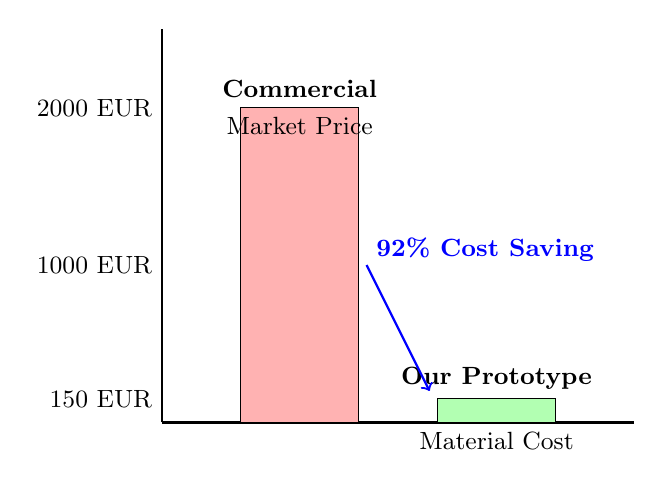
\begin{tikzpicture}[font=\small]
		% Axes
		\draw[thick] (0,0) -- (6,0); % X Axis
		\draw[thick] (0,0) -- (0,5); % Y Axis
		
		% Y-Axis Labels
		\node[anchor=east] at (0,4) {2000 EUR};
		\node[anchor=east] at (0,2) {1000 EUR};
		\node[anchor=east] at (0,0.3) {150 EUR};
		
		% Bar 1: Commercial System (Red)
		\draw[fill=red!30] (1,0) rectangle (2.5, 4);
		\node[above] at (1.75, 4) {\textbf{Commercial}};
		\node[below] at (1.75, 4) {Market Price};
		
		% Bar 2: Our Prototype (Green)
		\draw[fill=green!30] (3.5,0) rectangle (5, 0.3); % Scaled height (150/2000 * 4 approx 0.3)
		\node[above] at (4.25, 0.3) {\textbf{Our Prototype}};
		\node[below] at (4.25, 0) {Material Cost};
		
		% Annotation arrow
		\draw[->, thick, blue] (2.6, 2) -- (3.4, 0.4);
		\node[text=blue, anchor=west] at (2.6, 2.2) {\textbf{92\% Cost Saving}};
		
	\end{tikzpicture}
	\caption{Cost comparison between the Jetson-based prototype (150 EUR) and a standard Commercial ANPR unit (2000 EUR).}
	\label{fig:cost_chart}
\end{figure}

\section{Competitive Feature Analysis}
While cost is a significant advantage, operational capabilities must also be considered. Table \ref{tab:competitor_matrix} provides a direct feature comparison.

\begin{table}[H]
	\centering
	\caption{Feature Matrix: Prototype vs. Commercial Standard}
	\label{tab:competitor_matrix}
	\renewcommand{\arraystretch}{1.4}
	\begin{tabular}{|l|c|c|}
		\hline
		\textbf{Feature} & \textbf{Our Jetson Prototype} & \textbf{Commercial System} \\ \hline
		\textbf{Hardware Cost} & \textbf{Low (< 200 EUR)} & High (> 2000 EUR) \\ \hline
		\textbf{Data Privacy} & \textbf{Edge-Local (GDPR Safe)} & Cloud / Server Dependent \\ \hline
		\textbf{Customizability} & \textbf{Open Source (Python)} & Proprietary (Closed) \\ \hline
		\textbf{Night Vision} & Passive (Needs Streetlight) & \textbf{Active IR Illumination} \\ \hline
		\textbf{Deployment} & Portable / Battery Possible & Fixed Infrastructure \\ \hline
		\textbf{Billing Logic} & \textbf{Configurable Rules} & Standard Toll Only \\ \hline
	\end{tabular}
\end{table}

\textbf{Analysis:}
\begin{itemize}
	\item \textbf{Strengths:} Our system excels in flexibility and privacy. The open-source nature allows airport management to modify billing rules (e.g., changing the 15-minute free tier to 30 minutes) without paying vendor support fees.
	\item \textbf{Weaknesses:} The lack of active Infrared (IR) illumination limits performance in total darkness, a feature standard in commercial units.
\end{itemize}

\section{Project Roadmap (Future Work)}
To transition this TRL-4 (Lab Validation) prototype into a deployable TRL-7 product, a three-phase development roadmap is proposed.

\begin{table}[H]
	\centering
	\caption{Development Roadmap for Production Readiness}
	\label{tab:roadmap}
	\begin{tabular}{|l|l|l|}
		\hline
		\textbf{Phase} & \textbf{Timeline} & \textbf{Key Deliverables} \\ \hline
		\textbf{Phase 1: Hardware} & Months 1-3 & 
		\begin{minipage}[t]{6cm}
			\begin{itemize}
				\item Replace USB Webcam with MIPI-CSI Sensor.
				\item Design 3D-printed IP67 weatherproof enclosure.
				\item Integrate active IR LED illuminators.
			\end{itemize} 
		\end{minipage} \\ \hline
		
		\textbf{Phase 2: Payment} & Months 4-6 & 
		\begin{minipage}[t]{6cm}
			\begin{itemize}
				\item Integrate NFC Module (PN532) for card tapping.
				\item Connect to Stripe/PayPal API.
				\item Add thermal printer for physical receipts.
			\end{itemize} 
		\end{minipage} \\ \hline
		
		\textbf{Phase 3: Network} & Months 7-9 & 
		\begin{minipage}[t]{6cm}
			\begin{itemize}
				\item Develop "Fleet Dashboard" for remote management.
				\item Implement Over-the-Air (OTA) update mechanism.
				\item Sync "Stolen Car" database with police APIs.
			\end{itemize} 
		\end{minipage} \\ \hline
	\end{tabular}
\end{table}

\section{Final Remarks}
This project serves as a proof-of-concept for the democratization of Smart City infrastructure. We have proven that with \textbf{89.00 EUR} of hardware and modern neural networks, "Intelligence" is no longer a function of budget, but of optimization. The system stands ready for pilot testing in low-speed, controlled access environments such as private employee parking lots or residential gated communities.